\section{Instrumentos}\label{ins}
El conjunto de instrumentos se elabor\'o con los  siguientes recursos:
\begin{itemize}
\item Humanos
	\begin{itemize}
	\item Profesionales (entrenadores deportivos).
	\item Atletas
	\item Investigador
	\end{itemize}
\item No humanos
	\begin{itemize}
	\item Mesa de soporte con una altura de 0.70 metros.
	\item Cable de extensi\'on el\'ectrico de 2.00 metros. 
	\item Computadora port\'atil
		\begin{itemize}
		\item Conector de carga de alimentaci\'on
		\end{itemize}
	\item Sensor Kinect
		\begin{itemize}
		\item Adaptador del Kinect
		\end{itemize}
	\end{itemize}
\end{itemize}
\subsection{Formulario de registro de movimiento} \label{ins:frmMov}
Este formulario se adjunta en anexos (ver figura \ref{fig:frmWhiteMov}), la cual tiene como objetivo describir el movimiento v\'alido de cada equipo deportivo. Por otra parte, el formulario est\'a compuesto por los siguientes incisos:
\begin{itemize}
	\item \textbf{Nombre del movimiento:} Nombre que se identifica en gu\'ias deportivas o de salud.
	\item \textbf{Descripci\'on del movimiento: } Contesta la pregunta: ?`Qu\'e es el movimiento?
	\item \textbf{Movimiento unilateral:} Si es afirmativo, el movimiento trabaja con solo una parte del cuerpo (izquierda o derecha, ejemplo una patada), en caso contrario, se considera todas las partes del cuerpo (izquierda y derecha, ejemplo un salto).
	\item \textbf{Partes del cuerpo ignorada:} M\'ultiples respuestas que identifican las articulaciones ignoradas (debido que no es informaci\'on relevante para el movimiento):
	\begin{itemize}
		\item \textbf{Brazo derecho o izquierdo:} Ignora las siguientes articulaciones (seg\'un su lado): Pulgar, dedo del medio, mano, codo, hombro, centro de los hombros, cuello, cabeza y espalda.
		\item \textbf{Cuerpo inferior:} Ignora las siguientes articulaciones (en ambos lados): Centro de cadera, caderas, rodillas, tobillos y pies.
	\end{itemize}
		\item \textbf{N\'umero de pasos:} Cantidad de pasos del movimiento.
		\item \textbf{Offset del paso:} Valor que separa las etiquetas por partes iguales.
		\item \textbf{Valor de identificaci\'on:} Valor que reconoce las etiquetas por partes iguales.
		\item \textbf{Detalle por paso:} Muestra los pasos establecidos por el profesional, para ejecutar un movimiento v\'alido:
			\begin{itemize}
		\item \textbf{Paso:} N\'umero \'unico que identifica el paso.
		\item \textbf{Diagrama:} Imagen visual del paso (seguimiento del esqueleto).
		\item \textbf{Descripci\'on del paso:} Responde la pregunta: ?`Cu\'al es la postura del cuerpo durante ese paso?
		\item \textbf{Etiqueta:} N\'umero \'unico que identifica el paso a partir de la probabilidad de movimiento.
	\item \textbf{Rango de identificaci\'on:} Rango m\'aximo que identifica el paso dentro de la probabilidad del movimiento.
	\end{itemize}
\end{itemize}
\subsection{Formulario de registro de rutina} \label{ins:frmRout}
Formulario adjuntado en anexos (Ver figura \ref{fig:frmWhiteRout}), tiene como funci\'on identificar los ejercicios de calentamiento  previamente a realizar el movimiento seleccionado por cada equipo deportivo, adem\'as de estandarizar el n\'umero de repeticiones del movimiento por cada atleta, a partir de los siguientes puntos:
\begin{itemize}
	\item \textbf{Descripci\'on del calentamiento:} Detalla el tipo de calentamiento (calentamiento con tu propio peso, calentamiento dentro de un ambiente, calentamiento a partir de objetos).
	\item \textbf{Movimientos:} Lista los movimientos que se realizan durante el calentamiento (Validado por el formulario de registro de movimiento).
	\item \textbf{Series:} Cantidad de veces que debe realizar un atleta, un conjunto de repeticiones del movimiento.
	\item \textbf{Repeticiones:} Cantidad de repeticiones del movimiento.
	\item \textbf{Tiempo:} Duraci\'on del calentamiento.
	\item \textbf{Im\'agenes:} Fotograf\'ias tomadas durante el entrenamiento de cada equipo deportivo.
	\item \textbf{Nombre del movimiento:} Movimiento seleccionado por cada equipo deportivo  (validado por el formulario de registro de movimiento).
	\item \textbf{Rutina:} Describe el tipo de rutina para la captura de datos:
	\begin{itemize}
		\item \textbf{Por tiempo:} M\'axima cantidad de repeticiones del movimiento, durante un tiempo establecido.
		\item \textbf{Escaleras:} N\'umeros de repeticiones establecidas, separadas por series.
	\end{itemize}	
\end{itemize}
\subsection{Interfaces de usuarios} \label{ins:UI}
Aplicaciones que interact\'uan con el usuario para la recolecci\'on de datos, en donde se trabajan con  tres tipos:
\subsubsection{Windows presentation foundation (WPF)}
\label{ins:UI:wpf}
El desarrollador, \citeA{wpf2019}, menciona que este tipo de interfaz permite crear aplicaciones de escritorio con la tecnolog\'ia .NET, la cual es soportado desde Windows XP hasta la \'ultima versi\'on de Windows (Windows 10). Por lo tanto, en el presente proyecto se utiliz\'o este tipo de interfaz para la construcci\'on del seguimiento del esqueleto, generado por los siguientes kits de desarrollo de software:
\begin{itemize}
	\item \textbf{Windows inputs:} Herramienta que permite crear elementos de un formulario (e.g. botones, cajas de textos) \cite{wpfWindows2019}.
	\item \textbf{Windows media:} Herramientas que permiten renderizar el seguimiento del esqueleto en tiempo real a partir de pinceles, colores, formas y dibujos \cite{WindowMedia2019}.
	\item \textbf{Windows threading:} Herramientas que permiten crear temporizadores para la renderizaci\'on del seguimiento del esqueleto en un per\'iodo del tiempo (30 fotogramas por segundos) \cite{WindowThreading2019}.
	\item \textbf{Kinect:} Herramientas que permiten acceder a las funcionalidades del sensor \cite{WindowKinect2019}, tales:
	\begin{itemize}
					\item \textbf{Body frame reader:} Obtiene la informaci\'on del seguimiento del esqueleto.
				\item \textbf{Estado del sensor:} Activo, pausa, no detectado e inactivo.
				\item \textbf{Datos del Visual Gesture Builder:} Normalizaci\'on de datos del sensor del Kinect para el uso del modelo de reconocimiento de movimiento.
			\item \textbf{Joint type:} Enumeradores que listan las articulaciones del seguimiento del esqueleto (e.g. manos, codos, hombros).
			\item \textbf{Visualizaci\'on de los recursos de los fotogramas para Visual Gesture Builder:} Interpreta la base de datos de gesturas y posiciones de un movimiento (.gdb), a partir del algoritmo Random Forest Regression.
	\end{itemize}	 
\end{itemize}
A partir de los kits de desarrollo se crearon 2 aplicaciones para la captura de informaci\'on.
\paragraph{Detecci\'on de profundidad}\mbox{} \\ \label{ins:UI:wpf:depth}
Esta aplicaci\'on tiene como objetivo recolectar la distancia correcta de profundidad entre el atleta y el Kinect, tomando en cuenta una articulaci\'on de an\'alisis, adem\'as de la altura del usuario medida desde la cabeza hasta los pies, tal como se presenta en la imagen de la interfaz gr\'afica de detecci\'on de profundidad:
\begin{figure}[H]
	\caption{Interfaz gr\'afica de detecci\'on de profundidad entre el usuario y el sensor}
	\label{fig:appDepth}
	\centering
	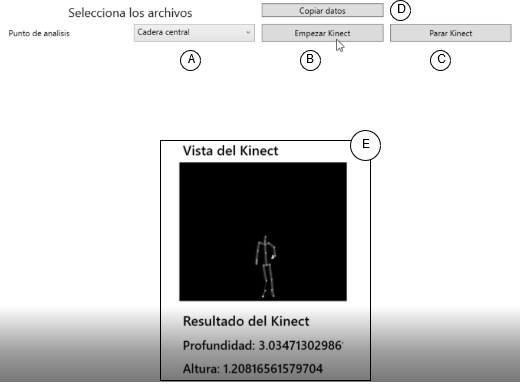
\includegraphics[width=380px,height=200px]{graphics/appProfundidad.png} \\
	\textbf{Fuente:} Propia.
\end{figure}
Esta interfaz se compone por 5 componentes:
\begin{enumerate}[A.]
    \item Selecci\'on de una articulaci\'on de an\'alisis.
    \item Bot\'on que empieza las funcionalidades del seguimiento del esqueleto.
    \item Bot\'on que finaliza las funcionalidades del seguimiento del esqueleto.
    \item Conjunto de paneles de controles que muestran una imagen en tiempo real del seguimiento del esqueleto, adem\'as de la altura (en metros) del usuario y la distancia de profundidad (en metros) entre el atleta y el sensor.
        \item Bot\'on que permite copiar a una hoja de observaci\'on (ver anexos, cuadro \ref{tab:obsDepth}) los siguientes datos respectivos: N\'umero de identificaci\'on de la articulaci\'on, la distancia de profundidad y la altura del usuario.
\end{enumerate}
\paragraph{Evaluaci\'on del movimiento}\mbox{} \\\label{ins:UI:wpf:evaluate}
Aplicaci\'on realizada por el autor del usuario, cuya funcionalidad es programar una rutina de tabata a partir del movimiento de cada equipo deportivo, mostrado en la interfaz gr\'afica de evaluaci\'on de un movimiento:
\begin{figure}[H]
	\caption{Interfaz gr\'afica de evaluaci\'on de un movimiento}
	\label{fig:appEvaluate}
	\centering
	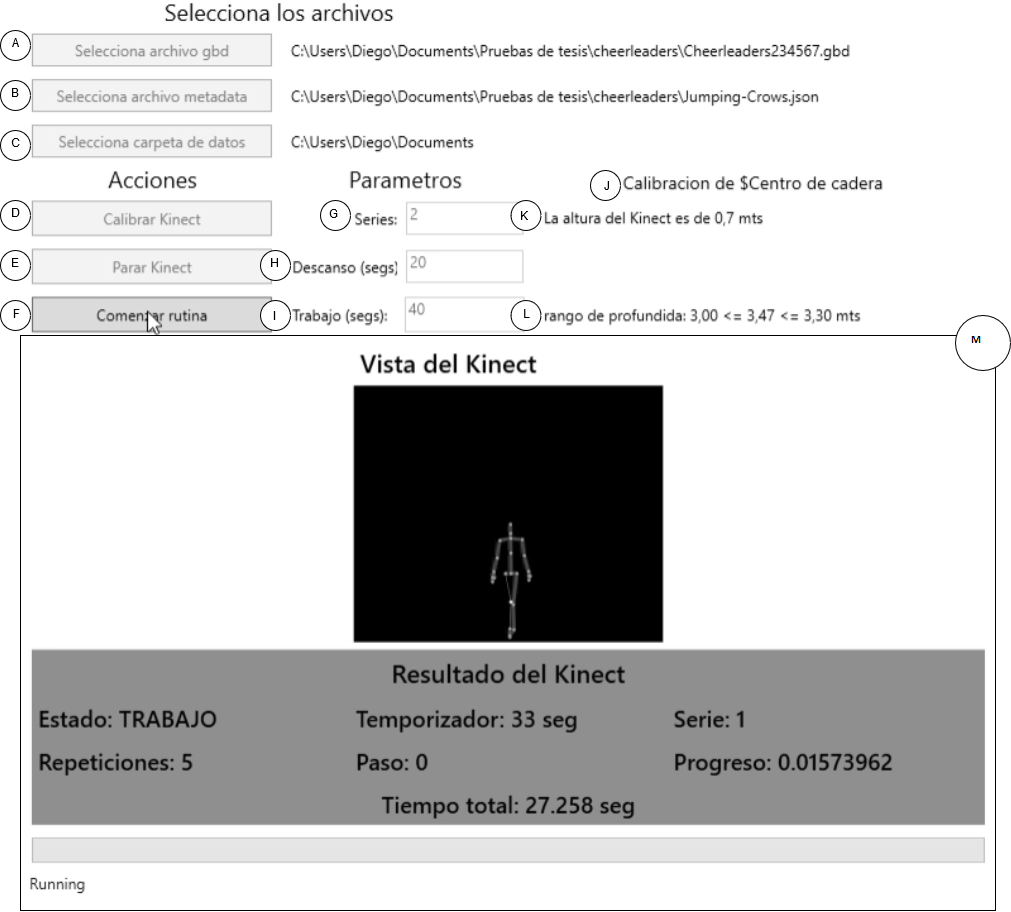
\includegraphics[width=380px,height=250px]{graphics/appEvaluacion.png} \\
	\textbf{Fuente:} Propia.
\end{figure}
Dicha interfaz se divide en 13 componentes:
\begin{enumerate}[A.]
    \item Bot\'on que permite seleccionar el archivo de base de datos del reconocimiento del movimiento.
    \item Bot\'on que permite seleccionar el archivo json que contiene toda la informaci\'on respectiva del movimiento (ver anexos, c\'odigo  \ref{code:jsonMeta}).
    \item Bot\'on que permite seleccionar la direcci\'on del archivo de resultado de tabata.
    \item Bot\'on que permite activar todas las funcionalidades del Kinect.    
    \item Bot\'on que permite detener todas las funcionalidades del Kinect. 
    \item Bot\'on que permite comenzar la rutina de tabata (en tiempo real).
   \item  Caja de texto num\'erica que indica la cantidad de tiempos de trabajos y descansos del atleta durante su rutina de tabata.
   \item  Caja de texto num\'erica que se\~nala el tiempo de descanso durante una rutina.
   \item  Caja de texto n\'umerica que muestra el tiempo de trabajo durante una rutina (durante este tiempo, el atleta debe realizar la cantidad m\'axima de repeticiones).
   \item  Etiqueta de articulaci\'on de an\'alisis para medir la distancia de profundidad entre el atleta y el sensor.
   \item  Etiqueta de la altura  recomendada (en metros)  del sensor y el suelo.
      \item  Etiqueta de la distancia m\'inima y m\'axima de profundidad del atleta con respecto al sensor, y por otra parte indica la distancia profundidad actual del usuario y el sensor.
      \item Conjunto de paneles de controles que muestran:
      \begin{itemize}
            \item  El seguimiento del esqueleto en tiempo real.
            \item  Estado actual de la rutina: Inicio, trabajo, descanso y fin.
            \item  Temporizador de cuenta regresiva del tiempo de trabajo o descanso (en segundos).
             \item  Serie actual que est\'a trabajando el atleta.
             \item  Contador de repeticiones de la serie actual.
              \item \'Ultimo paso ejecutado por el atleta (comenzando desde 0).   
             \item  Valor de probabilidad del movimiento (factor del movimiento).
             \item  Temporizador que mide el tiempo    empleado en la rutina (en segundos).
      \end{itemize}
\end{enumerate}
Ya definido los componentes de la interfaz, se debe tomar en cuenta que al finalizar cada rutina tabata  el programa genera un archivo json (ver anexos, c\'odigo  \ref{code:tabata}), con los siguientes resultados:
\begin{itemize}
	\item \textbf{Analizador de variables:} Indica las variables que fueron configurado en un tabata: Tiempo de descanso, tiempo de trabajo y la cantidad de series.
	\item  \textbf{Resultados generales:} Muestran los resultados del volumen de repeticiones  y el tiempo total empleado en la rutina de tabata.
	\item  \textbf{Resistencia:} Vector de informaci\'on que permite construir la gr\'afica de la rutina tabata, a partir de los siguientes par\'ametros:
	   \begin{itemize}  
   	\item \textbf{Uid:} C\'odigo \'unico de identificaci\'on de la gr\'afica.
   	\item \textbf{Label:} Nombre de la gr\'afica.
   	\item \textbf{Show line:} Condici\'on que permite dibujar la l\'inea de la tendencia de la gr\'afica.
    \item \textbf{Data:} Vector de datos que conforma la gr\'afica, en donde los datos del eje x, representan el tiempo de rutina (en segundos), y los datos del eje y, significan las repeticiones acumulada durante ese tiempo de rutina.
   \end{itemize}     
    \item \textbf{Potencia:} Cantidad de repeticiones m\'axima del movimiento, en el menor tiempo posible.
    \item \textbf{Velocidad:} Se divide en dos resultados:
           \begin{itemize}
       \item Cantidad promedio de repeticiones en una serie.
       \item Tiempo promedio por una repetici\'on
       \end{itemize}
\end{itemize} 
\subsubsection{Web}\mbox{} \\
\label{ins:UI:web}
Interfaz de usuario que permite capturar la informaci\'on de los formularios de movimiento, a partir de la siguiente arquitectura:
\begin{figure}[H]
	\caption{Arquitectura web}
	\label{fig:architectureWeb}
	\centering
	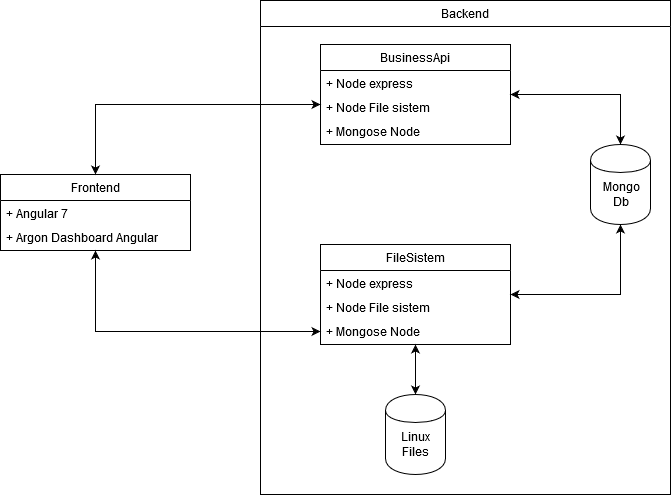
\includegraphics[width=430px,height=220px]{graphics/webArchitecture.PNG} \\
	\textbf{Fuente:} Propia.
\end{figure}
\begin{itemize}
\item Frontend
	\begin{itemize}
	\item \textbf{Web}: Interfaz agradable para el usuario, cuya finalidad es realizar llamadas a las aplicaciones de negocio y servidor de archivos.
	\end{itemize}
\item Backend
	\begin{itemize}
	\item \textbf{Business api:} Maneja todas las  funciones l\'ogicas del giro de negocios (e.g. Insertar movimiento, leer movimiento, resultados de rutina).
	\item \textbf{File sistem:} Interfaz de programaci\'on de aplicaciones que se encarga de almacenar los archivos de metadata que define una base de datos del movimiento.
		\item \textbf{Server files:} Servidor encargado de almacenar los archivos de bases de datos del movimiento v\'alido (.gdb) y sus respectivos v\'ideos (.xef).
		\item \textbf{Mongo DB:} Servidor de bases de datos no relacional, que se encarga de almacenar informaci\'on de la metadata del movimiento.
	\end{itemize}
\item Entornos de trabajo
\begin{itemize}
\item \textbf{Angular 7:} Herramienta que facilita la creaci\'on y el mantenimiento de una aplicaci\'on web \cite{angular2019}.
\item \textbf{Argon dashboard angular:} Herramienta  que facilita realizar una aplicaci\'on responsiva (adaptable a cualquier dispositivo a partir de un navegador web) \cite{argonDash}.
\item \textbf{Express js:} Herramienta encargada de realizar la comunicaci\'on entre aplicaciones, a partir del \acrlong{HTTP} \cite{fileSistem2019}.
\item \textbf{Mongoose:} Herramienta encargada de realizar cualquier operaci\'on de la base de datos de mongo (e.g. conexi\'on, recuperar datos, modificar registros) \cite{mongoose2019}.
\end{itemize}
\end{itemize}
As\'i mismo la aplicaci\'on web est\'a conformada por 4 vistas:
\paragraph{Vista del listado de movimientos}\mbox{} \\ \label{ins:UI:web:index}
Vista principal que muestra al usuario todos los movimientos que se han insertado en la base de datos.
\begin{figure}[H]
	\caption{Vista de listado de movimientos}
	\label{fig:viewIndex}
	\centering
	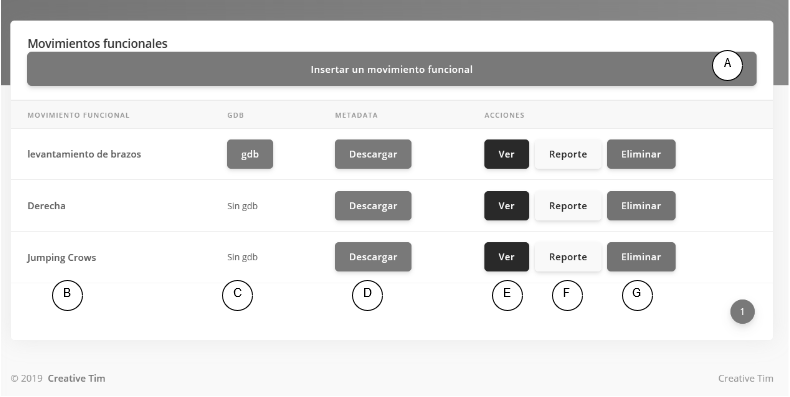
\includegraphics[width=440px,height=270px]{graphics/web-index.PNG} \\
	\textbf{Fuente:} Propia.
\end{figure}
\begin{enumerate}[A.]
\item Bot\'on que dirige al usuario a la pantalla de insertar un movimiento (Ver vista de creaci\'on de un movimiento).
\item Etiqueta que indica el nombre del movimiento.
\item Bot\'on que descarga el archivo de base de datos de un movimiento.
\item Bot\'on que exporta el archivo de metadata de un movimiento (Ver anexos, c\'odigo \ref{code:jsonMeta}), con los siguientes atributos:
	\begin{itemize}
	\item \textbf{Steps}: Vector num\'erico que contiene las etiquetas de cada paso de un movimiento.
	\item \textbf{Angles of movement}: Vector num\'erico que almacena los \'indices de cada articulaci\'on que interact\'uan en el movimiento.
	\item \textbf{Recognition}: Valor que construye  el rango de confiabilidad para detectar un paso de un movimiento.
	\item \textbf{Id}: C\'odigo \'unico que identifica el movimiento en la base de datos.
	\item \textbf{Height}: Altura del Kinect con respecto al suelo (medida en metros).	
	\item \textbf{Depth min}: Distancia m\'inima de profundidad del sensor y el atleta (medida en metros).
	\item \textbf{Depth max}: Distancia m\'axima de profundidad del sensor y el atleta (medida en metros).
	\item \textbf{Time stamp}: Fecha en la cual fue insertado el registro del movimiento.
	\item \textbf{Focus join}: Articulaci\'on de an\'alisis que permite medir la distancia de profundidad. 
	\end{itemize}
\item Bot\'on que dirige al usuario a la pantalla de detalle de un movimiento (ver vista de lectura de un movimiento).
\item Bot\'on que dirige al usuario a la pantalla de reporte de un movimiento (ver vista de resultados de un movimiento).
\item Bot\'on que elimina el registro del movimiento de la base de datos.
\end{enumerate}
\paragraph{Vista de creaci\'on de un movimiento}\mbox{} \\ \label{ins:UI:web:create}
Vista que se encarga de insertar toda la informaci\'on del movimiento, recuperada por los formularios.
\begin{figure}[H]
	\caption{Vista de crear un movimiento}
	\label{fig:viewCreate}
	\centering
	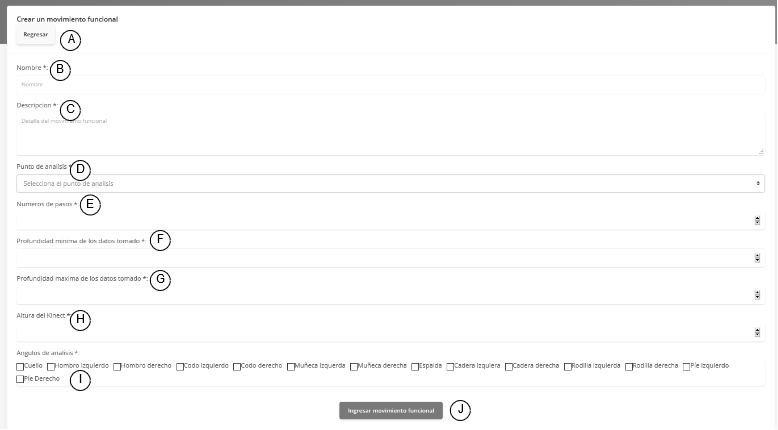
\includegraphics[width=460px,height=320px]{graphics/web-create.PNG} \\
	\textbf{Fuente:} Propia.
\end{figure}
\begin{enumerate}[A.]
\item Bot\'on que dirige al usuario a la pantalla del listado de los movimientos (ver vista de listado de movimientos).
\item Caja de texto para ingresar el nombre del movimiento (Recuperado del formulario de registro de movimiento, atributo de nombre).
\item Caja de texto para ingresar el detalle del movimiento (Recuperado del formulario de registro de movimiento, atributo de descripci\'on).
\item Selecci\'on de la articulaci\'on de an\'alisis (recuperado de la aplicaci\'on de detecci\'on de profundidad, atributo de articulaci\'on de an\'alisis).
\item Caja de texto num\'erica que ingresa la cantidad de pasos del movimiento (recuperado del formulario de registro de movimiento, atributo de n\'umero de pasos).
\item Caja de texto num\'erica que ingresa la distancia m\'inima de profundidad (ver formula \ref{frm:maxDepth}).
\item Caja de texto num\'erica que ingresa la distancia m\'axima de profundidad (ver formula \ref{frm:minDepth}).
\item Caja de texto num\'erica que ingresa la altura del Kinect con respecto al suelo (para el presente proyecto es de 0.70 metros, debido que es la altura de la mesa que daba soporte al sensor).
\item Listado m\'ultiples de articulaciones que intervienen en el movimiento (recuperado del formulario de registro de rutinas, atributo de articulaciones no ignoradas).
\item Bot\'on que almacena toda la informaci\'on respectiva del formulario web.
\end{enumerate}
\paragraph{Vista de lectura de un movimiento}\mbox{} \\ \label{ins:UI:web:read}
Vista que se encarga de mostrar toda la informaci\'on del movimiento, adem\'as de insertar el archivo de base de datos de gesturas y modificar el rango de confiabilidad de reconocimiento de pasos.
\begin{figure}[H]
	\caption{Vista de lectura del movimiento}
	\label{fig:viewRead}
	\centering
	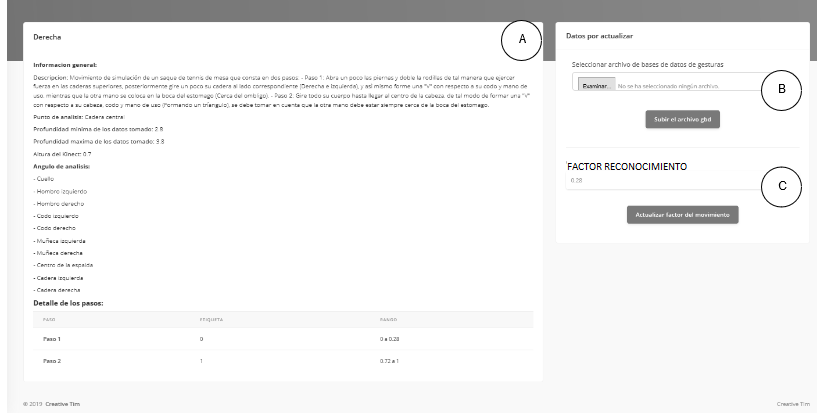
\includegraphics[width=460px,height=320px]{graphics/web-read.PNG} \\
	\textbf{Fuente:} Propia.
\end{figure}
\begin{enumerate}[A.]
\item Ficha de informaci\'on que detalla todas las caracter\'isticas del movimiento (e.g. Nombre, descripci\'on, etiquetas de los pasos, intervalos de confianza de los pasos, articulaciones del movimiento).
\item Conjuntos de controladores que permiten seleccionar un archivo de base de datos de gesturas y almacenarlo en el servidor de archivos.
\item Conjunto de controladores que permiten cambiar el valor del factor de reconocimiento (Ver ecuaci\'on \ref{frm:rangoConfiabilidad}).
\end{enumerate}
\paragraph{Vista de resultados de un movimiento}\mbox{} \\ \label{ins:UI:web:result}
Vista que expone los resultados de la aplicaci\'on de evaluaci\'on de un movimiento:
\begin{figure}[H]
	\caption{Resultados de la rutina tabata de un movimiento}
	\label{fig:resultsTabata}
	\centering
	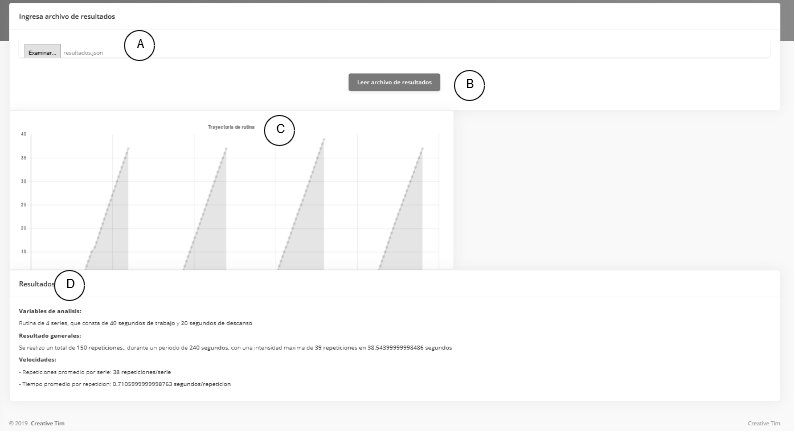
\includegraphics[width=460px,height=320px]{graphics/web-results.PNG} \\
	\textbf{Fuente:} Propia.
\end{figure}
\begin{enumerate}[A.]
\item Conjuntos de controladores que seleccionan y leen un archivo de resultados de la rutina tabata (ver anexos, c\'odigo \ref{code:tabata}).
\item Diagrama de dispersi\'on de la rutina tabata, la cual muestra las repeticiones acumuladas durante tiempos de trabajos y de descansos.
\item Ficha informativa que muestra los resultados de la rutina tabata (e.g. Variables que fueron configuradas en el tabata, volumen de repeticiones, duraci\'on de la rutina, repeticiones por serie de trabajo, tiempo promedio por repetici\'on).
\end{enumerate}
\subsubsection{Consola (Windows)}\mbox{} \\ \label{ins:cons}
\begin{figure}[H]
	\caption{Aplicaci\'on de extracci\'on de datos en los v\'ideos (xef)}
	\label{fig:appConsole}
	\centering
	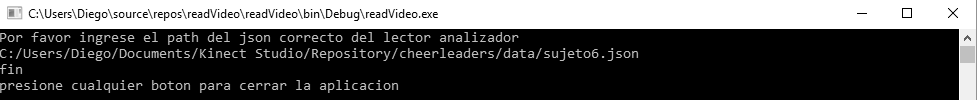
\includegraphics[width=460px,height=50px]{graphics/appConsole.PNG} \\
	\textbf{Fuente:} Propia.
\end{figure} 
Aplicaci\'on de consola que permite extraer informaci\'on de los v\'ideos (.xef) y generar una hoja de observaciones del seguimiento de esqueleto (ver anexo, tabla \ref{tab:obsVideoData}), con la ayuda de las siguientes herramientas:
\begin{itemize}
\item \textbf{System console:} Permite utilizar todas las funcionalidades de consola de windows \cite{windowConsole2019}.
\item \textbf{System io:} Proporciona todas las  funcionalidades de manejo de archivos \cite{windowIO2019}.
\item \textbf{Kinect xef tools:} Librer\'ia que extrae de los v\'ideos (xef), la posici\'on de cada articulaci\'on del seguimiento del tiempo, durante un per\'iodo del tiempo \cite{kinectXEFTools}.
\end{itemize}
Para el funcionamiento de la aplicaci\'on, es necesario un archivo de lector analizador (ver anexos, c\'odigo \ref{code:jsonVideo}), en donde est\'a conformado por los siguientes atributos:
\begin{itemize}
\item \textbf{Path video:} Direcci\'on del archivo  de v\'ideo a analizar (.xef).
\item \textbf{Path write:} Direcci\'on del archivo  resultante (.csv).
\item \textbf{Joints:} Vector num\'erico que muestra los \'indices de las articulaciones que se desean extraer la informaci\'on.
\item \textbf{Frame data:} Vector de vectores de cadenas, la cual por cada vector de cadena se indica el segmento de v\'ideo de extracci\'on de datos (punto de inicio y punto final).
\end{itemize}
\subsection{Kinect configuration verifier} \label{ins:KinectCheckt}
Herramienta del kit de desarrollo de software del sensor del Kinect, que tiene como objetivo  analizar la computadora que se encuentra conectado al sensor, verificando las compatibilidades del hardware (e.g. procesador, controlador de usb, sistema operativo, conexi\'on del sensor), adem\'as de chequear la comunicaci\'on con la c\'amara (e.g. canales de color y de profundidad).
\subsection{Kinect studio} \label{ins:KinectStudio}
Herramienta del kit de desarrollo de software del sensor del Kinect que se utiliza para monitorear, grabar (V\'ideos .xef) y reproducir datos de la c\'amara \cite{KinectStudio2019}, a partir de los siguientes canales:
\begin{figure}[H]
	\caption{Canales por defecto para grabar un v\'ideo en Kinect studio }
	\label{fig:streamDefault}
	\centering
	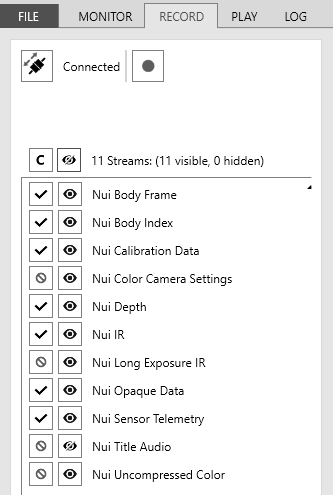
\includegraphics[width=200px,height=360px]{graphics/streamsRecord.PNG} \\
	\textbf{Fuente:} Propia.
\end{figure} 
\begin{itemize}
\item Activos:
\begin{itemize}
\item \textbf{NUI body frame:} Encargado de los datos con relaci\'on al seguimiento del esqueleto.
\item \textbf{NUI body Index:} Identifica de 1 a 6 esqueletos con su respectivo \'indice.
\item \textbf{NUI calibration data:} Responsable de obtener la mayor precisi\'on de datos.
\item \textbf{NUI depth:} Controla y obtiene los datos de profundidad.
\item \textbf{NUI ir:} Monitoreo de los sensores de profundidad.
\item \textbf{NUI opaque data:} Disminuye el ruido de la luz.
\item \textbf{NUI sensor telemetry:} Encargado de actualizar y obtener nuevos datos en un per\'iodo de tiempo.
\end{itemize}
\item Inactivos:
\begin{itemize}
\item \textbf{NUI color camera settings:} Encargado de la conversi\'on de colores (e.g. YUV o RGB)
\item \textbf{NUI long exposure ir:} Identifica  objetos externos al seguimiento del esqueleto (e.g. mesa, pelota, pesa).
\item \textbf{NUI uncompressed color:} Responsable de obtener los datos de color (e.g. c\'odigo de colores de un sem\'aforo).
\end{itemize}
\end{itemize}
As\'i mismo esta herramienta proporciona una interfaz gr\'afica para ver y analizar los v\'ideos a partir de segmentos (parte de inicio y fin) y puntos de pausas.
\begin{figure}[H]
	\caption{Lectura de v\'ideo .xef }
	\label{fig:readVideoXEF}
	\centering
	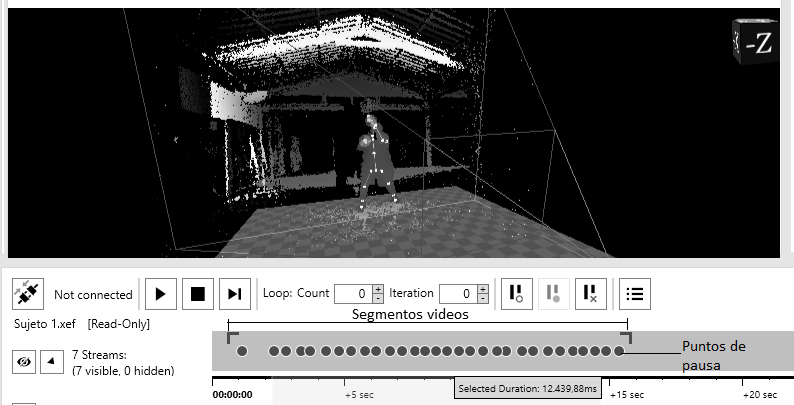
\includegraphics[width=460px,height=320px]{graphics/readVideo.PNG} \\
	\textbf{Fuente:} Propia.
\end{figure} 
\subsection{Visual Gesture Builder} \label{ins:VisualGestureBuilder}
Herramienta que genera datos para la detecci\'on de gestos en tiempo de ejecuci\'on, usando tecnolog\'ias de m\'aquinas de aprendizaje (Random Forest Regression), con el fin objetivo de reconocer un gesto (e.g. saltar, bailar, sentarse) \cite{KinectBuilder2019}, a trav\'es de la etiquetaci\'on de fotogramas y la configuraci\'on de las siguientes variables:
 \begin{figure}[H]
	\caption{Variables de configuraci\'on de Visual Gesture Builder}
	\label{fig:visualGesture}
	\centering
	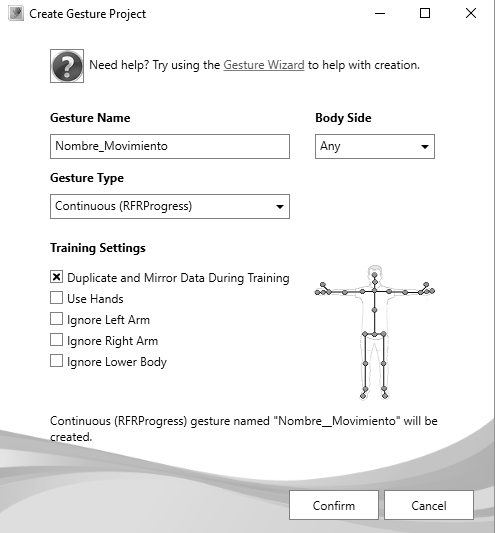
\includegraphics[width=300px,height=300px]{graphics/settingsGesture.PNG} \\
	\textbf{Fuente:} Propia.
\end{figure} 
\begin{itemize}
\item \textbf{Gesture name:} Nombre del movimiento  (Recuperado del formulario de registro de movimiento, atributo de nombre).
\item \textbf{Body side:} Valor por defecto es  ninguno, debido que no importa el lado que se est\'a ejecutando el movimiento, en caso que sea un movimiento unilateral, el modelo replica un modelo espejo, por ejemplo una patada lateral derecha es la replica de una patada lateral izquierda.
\item \textbf{Gesture type:} El valor por defecto es RFRProgress (Algoritmo de Random Forest Regression), debido que est\'a analizando movimiento continuos (e.g. salto, patada, saque).
\item \textbf{Duplicate and mirror data during training:} Se selecciona, si no es un \gls{MovUni} (Ver formulario de registro de movimiento, atributo unilateral), debido que replica datos de lado izquierdo al lado derecho y viceversa, por ejemplo en un salto.
\item \textbf{User hand:} El valor de defecto es falso, debido que no se est\'a analizando el agarre de la mano ante un objeto (e.g. bal\'on, pesa, raqueta).
\item \textbf{Ignore part body:} Se activan  aquellas partes del cuerpo que se desean ignorar durante el movimiento (Ver formulario de registro de movimiento, articulaciones ignoradas).
\end{itemize}
Luego de configurar las variables globales, el proyecto crear\'a una base de datos de gesturas vac\'io, la cual debe adjuntar todos los v\'ideos (.xef)  y por cada v\'ideo se debe etiquetar los valores de fotogramas (Seg\'un los pasos definido en el formulario de registro de movimiento), con el fin objetivo de: 
\begin{itemize}
\item \textbf{Construir:} Acci\'on que entrena y genera el modelo a partir de un archivo de base de datos de gesturas (.gbd).
\item \textbf{Analizar:} Funci\'on que permite seleccionar archivos de base de datos de gesturas y posteriormente compararlo con v\'ideos previamente etiquetados, encontrando el valor real (valor de la etiqueta) y el valor pron\'osticado del modelo (estos valores son usado para completar la hoja de observaci\'on de errores modelo, ver anexos, tabla \ref{tab:obsErrores}).
\end{itemize}
\subsection{Herramienta para el an\'alisis de datos} \label{ins:toolsAn}
Se utiliz\'o el software Microsoft Excel, para la tabulaci\'on y organizaci\'on de los datos.